
\chapter{Kravspecifikation}
\section{Godkendelsesformular}
\begin{table}[h!]
\label{tab:tabel2}
\begin{tabular}{| l | >{\raggedright\arraybackslash}p{12cm} |}
   \hline
   \textbf{Forfattere} & Line, Mette, Brian, Mohamed, Khaled og Ida\\ \hline
   \textbf{Godkendes af:} & Samuel Alberg Thrysøe\\ \hline
   \textbf{Antal sider:} & \\ \hline
   \textbf{Kunde:} & IHA\\ \hline
\end{tabular}
\end{table}
\textbf{Ved underskrivelse af dette dokument accepteres det af begge parter, som værende kravene til udviklingen af det ønskede system.}
\newline
\textbf{Sted og dato:}\\
\\
\\
\begin{table}
[h!]
\begin{tabular}{ l lllllllll l}
--------------------------------------&&&&&&&&&&--------------------------------------\\ 
Kundens underskrift &&&&&&&&&&Leverandørens underskrift\\
\end{tabular}
\end{table}
\section{Indledning}

\newpage

\section{Systembeskrivelse}

\newpage

\section{Aktør-kontekst diagram}
\begin{figure}[h!]
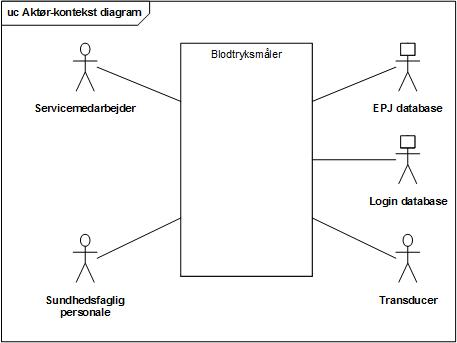
\includegraphics[width =0.8\textwidth , left]{billeder/Aktorkontekst.jpg}
\end{figure}

\newpage


\section{Use cases}
\begin{figure}[h!]
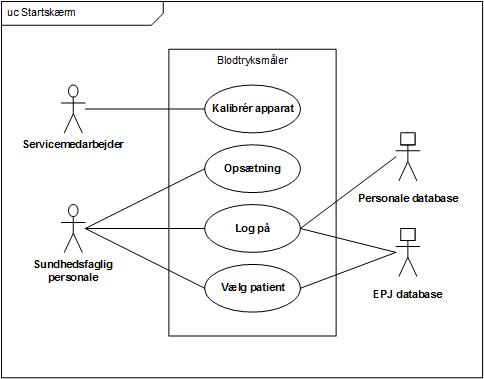
\includegraphics[width =0.7\textwidth , center]{billeder/UCStart}
\end{figure}
\begin{figure}[h!]
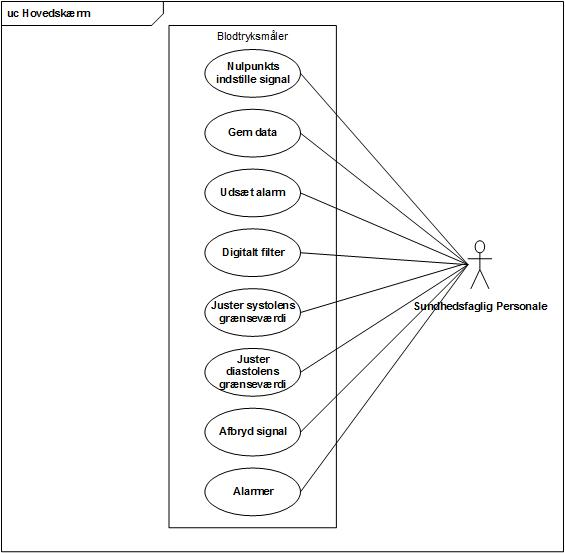
\includegraphics[width =0.8\textwidth , center]{billeder/UChoved}
\end{figure}
\newpage
\begin{table}[H]
\caption{Use case 1}\label{tab:tabel3}
\begin{tabular}{| l | >{\raggedright\arraybackslash}p{11cm} |}
   \hline
   \textbf{Use case 1} & \textbf{Kalibrer apparat}\\ \hline
   Mål: & Få kalibreret apparatet \\ \hline
   Initiering: & Startes af Servicemedarbejder\\ \hline
   Aktører:& Servicemedarbejder (primær)\\ \hline
   Referencer: & - \\ \hline
   Samtidige forekomster: & én kalibrering pr. apparat \\\hline
   Forudsætninger: & Blodtryksmålersystemet er tændt og tilsluttet kalibreringsudstyret.\\ \hline
   Resultat:& Apparatet er kalibreret\\ \hline
   Hovedscenarie:& 
1. Tryk på "Kalibrering"\newline
2. Systemet starter kalibreringen\newline
3. Besked: "Kalibreringen er fuldendt" vises på GUI\\\hline
Udvidelse/undtagelser: & - \\\hline
\end{tabular}
\end{table}

\begin{table}[H]
\caption{Use case 2}\label{tab:tabel3}
\begin{tabular}{| l | >{\raggedright\arraybackslash}p{11cm} |}
   \hline
   \textbf{Use case 2} & \textbf{Opsætning}\\ \hline
   Mål: & Få valgt port til NI-DAQ \\ \hline
   Initiering: & startes af Sundhedsfaglig personalee\\ \hline
   Aktører:& Sundhedsfaglig personale (primær) \\ \hline
   Referencer: &  -\\ \hline
   Samtidige forekomster: & Ét blodtryksmålersystem pr. opsætning \\\hline
   Forudsætninger: & Systemet tilsluttet en computer og tændt. \\ \hline
   Resultat:& Port valgt\\ \hline
   Hovedscenarie:& 
1. Tryk på opsætnings dropdown på startskærmen\newline
2. Port vælges \\\hline
Udvidelse/undtagelser: & -\\\hline
\end{tabular}
\end{table}



\begin{table}[H]
\caption{Use case 3}\label{tab:tabel3}
\begin{tabular}{| l | >{\raggedright\arraybackslash}p{11cm} |}
   \hline
   \textbf{Use case 3} & \textbf{Log på}\\ \hline
   Mål: & Den sundhedsfaglige få logget på "EPJ"-systemet \\ \hline
   Initiering: & Startes af Sundhedsfaglig personale\\ \hline
   Aktører:& Sundhedsfaglig personale (primær)\\ \hline
   Referencer: & Use case 2 \\ \hline
   Samtidige forekomster: & Én sundhedsfaglig pr. system \\\hline
   Forudsætninger: & Use case 2: Opsætning, er kørt succesfuldt\\ \hline
   Resultat:& Den sundhedsfaglige er logget på\\ \hline
   Hovedscenarie:& 
1. Indtast brugernavn og kode\newline
2. Tryk på "Login"\newline
   $[$Undtagelse 1: Brugernavn og/eller kode indtastet forkert$]$\\\hline
Udvidelse/undtagelser: & $[$Undtagelse 1: Brugernavn og/eller kode indtastet forkert$]$\newline
1.1 Besked: "Brugernavn og/eller kode indtastet forkert"\newline
1.2 Use case 3 starter forfra \\\hline
\end{tabular}
\end{table}



\begin{table}[H]
\caption{Use case 4}\label{tab:tabel3}
\begin{tabular}{| l | >{\raggedright\arraybackslash}p{11cm} |}
   \hline
   \textbf{Use case 4} & \textbf{Vælg patient}\\ \hline
   Mål: & Få valgt patienten og skiftet til hovedskærmen \\ \hline
   Initiering: & Startes af Sundhedsfaglig personale\\ \hline
   Aktører:& Sundhedsfaglig personale (primær)\\ \hline
   Referencer: & Use case 3 \\ \hline
   Samtidige forekomster: & - \\\hline
   Forudsætninger: & Use case 3: Log på, er kørt succesfuldt.\\ \hline
   Resultat:& Patient valgt og kommet til hovedskærmen.\\ \hline
   Hovedscenarie:& 
1. Tryk på dropdrow på startskærm \newline
2. Vælg patienten og dobbeltklik på denne \newline
3. Hovedskærmen kommer frem  \\\hline
Udvidelse/undtagelser: & - \\\hline
\end{tabular}
\end{table}



\begin{table}[H]
\caption{Use case 5}\label{tab:tabel3}
\begin{tabular}{| l | >{\raggedright\arraybackslash}p{11cm} |}
   \hline
   \textbf{Use case 5} & \textbf{Start signal}\\ \hline
   Mål: & Få startet målingen \\ \hline
   Initiering: & Startes af Sundhedsfaglig personale\\ \hline
   Aktører:& Sundhedsfaglig personale (primær), Transducer (sekundær)\\ \hline
   Referencer: & Use case 4\\ \hline
   Samtidige forekomster: & Én transducer pr. måling  \\\hline
   Forudsætninger: & Use case 4: Vælg patient, er kørt succesfuldt og transduceren er tilsluttet\\ \hline
   Resultat:& Transducerens data vises i GUI \\ \hline
   Hovedscenarie:& 
1. Tryk på "Start"\newline
2. Systemet indhenter data og starter timer\newline
3. EKG, arterietryk og iltmætningskurve præsenteres kontinuert på hver sin graf. Puls, systole, diastole, middeltryk og iltmætning vises som talværdier på GUI. Data gemmes automatisk i database.\\\hline
Udvidelse/undtagelser: & - \\\hline
\end{tabular}
\end{table}


\begin{table}[H]
\caption{Use case 6}\label{tab:tabel3}
\begin{tabular}{| l | >{\raggedright\arraybackslash}p{11cm} |}
   \hline
   \textbf{Use case 6} & \textbf{Nulpunkts indstille signal}\\ \hline
   Mål: & Få nulpunkts indstillet signalerne, sådan at signalerne ligger korrekte på deres akse. \\ \hline
   Initiering: & Startes af Sundhedsfaglig personale\\ \hline
   Aktører:& Sundhedsfaglig personale (primær)\\ \hline
   Referencer: & Use case 5\\ \hline
   Samtidige forekomster: & -  \\\hline
   Forudsætninger: & Use case 5: Start signal, er kørt succesfuldt\\ \hline
   Resultat:& Signalet er nulpunkts indstillet\\ \hline
   Hovedscenarie:& 
1. Tryk på "Nulpunks indstilling"\newline
2. Systemet starter nulpunkts indstillingen\newline
3. Besked "Nulpunkts indstillingen er fuldent" vises på GUI\\\hline
Udvidelse/undtagelser: & - \\\hline
\end{tabular}
\end{table}


\begin{table}[H]
\caption{Use case 7}\label{tab:tabel3}
\begin{tabular}{| l | >{\raggedright\arraybackslash}p{11cm} |}
   \hline
   \textbf{Use case 7} & \textbf{Udsæt alarm}\\ \hline
   Mål: & Få udsat alarmens lyd i et minut \\ \hline
   Initiering: & Startes af Sundhedsfaglig personale\\ \hline
   Aktører:& Sundhedsfaglig personale (primær) \\ \hline
   Referencer: & Use case 11 \\ \hline
   Samtidige forekomster: & \\\hline
   Forudsætninger: & Use case 11: Alarmer, er igangsat \\ \hline
   Resultat:& Alarmens lyd er stoppet et minut\\ \hline
   Hovedscenarie:& 
1. Tryk på "Udsæt alarm"\newline
2. Systemet stopper alarmens lyd i et minut \\\hline
Udvidelse/undtagelser: & -\\\hline
\end{tabular}
\end{table}

\begin{table}[H]
\caption{Use case 8}\label{tab:tabel3}
\begin{tabular}{| l | >{\raggedright\arraybackslash}p{11cm} |}
   \hline
   \textbf{Use case 8} & \textbf{Digitalt filter}\\ \hline
   Mål: &  Få slået det digitale filter til eller fra \\ \hline
   Initiering: & Startes af Sundhedsfaglig personale\\ \hline
   Aktører:& Sundhedsfaglig personale (primær)\\ \hline
   Referencer: & Use case 5 \\ \hline
   Samtidige forekomster: & - \\\hline
   Forudsætninger: & Use case 5: Start signal, er kørt succesfuldt\\ \hline
   Resultat:& Det digitale filter er slået til eller fra\\ \hline
   Hovedscenarie:& 
1. Tryk på "Digitalt filter OFF" \newline
2. Systemet slår det digitale filter fra\newline
3. Tryk på "Digitalt filter ON"\newline
4. Systemet slår det digitale filter til\\\hline
Udvidelse/undtagelser: & -\\\hline
\end{tabular}
\end{table}

\begin{table}[H]
\caption{Use case 9}\label{tab:tabel3}
\begin{tabular}{| l | >{\raggedright\arraybackslash}p{11cm} |}
   \hline
   \textbf{Use case 9} & \textbf{Juster systolens grænseværdi}\\ \hline
   Mål: & Få flyttet grænseværdi intervallet for systolen op eller ned \\ \hline
   Initiering: & Startes af Sundhedsfaglig personale\\ \hline
   Aktører:& Sundhedsfaglig personale (primær)\\ \hline
   Referencer: & Use case 5 \\ \hline
   Samtidige forekomster: & \\\hline
   Forudsætninger: & Use case 5: Start signal, er kørt succesfuldt\\ \hline
   Resultat:& Grænseværdi intervallet for systolen er justeret og intervals værdierne vises i GUI. \\ \hline
   Hovedscenarie:& 
1. Tryk på "Systole op"\newline
2. Grænseværdien ændres 2.5mmHg op og intervallet vises i GUI\newline
3. Tryk på "Systole ned"\newline
4. Grænseværdien ændres 2.5mmHg ned og intervallet vises i GUI\\\hline
Udvidelse/undtagelser: & -\\\hline
\end{tabular}
\end{table}

\begin{table}[H]
\caption{Use case 10}\label{tab:tabel3}
\begin{tabular}{| l | >{\raggedright\arraybackslash}p{11cm} |}
   \hline
   \textbf{Use case 10} & \textbf{Juster diastolens grænseværdi}\\ \hline
   Mål: &  Få flyttet grænseværdi intervallet for diastolen op eller ned\\ \hline
   Initiering: & Startes af Sundhedsfaglig personale \\ \hline
   Aktører: & Sundhedsfaglig personale (primær) \\ \hline
   Referencer: & Use case 5\\ \hline
   Samtidige forekomster: & - \\\hline
   Forudsætninger: & Use case 5: Start signal, er kørt succesfuldt\\ \hline
   Resultat:& Grænseværdi intervallet for diastolen er justeret og intervals værdierne vises i GUI.\\ \hline
   Hovedscenarie:& 
1. Tryk "Diastole op"\newline
2. Diastolens grænseværdi ændres 2.5mmHg op og intervallet vises i GUI\newline
3. Tryk "Diastole ned"\newline
4. Diastolens grænseværdi ændres 2.5mmHg ned og intervallet vises i GUI\\\hline
Udvidelse/undtagelser: & -\\\hline
\end{tabular}
\end{table}

\begin{table}[H]
\caption{Use case 11}\label{tab:tabel3}
\begin{tabular}{| l | >{\raggedright\arraybackslash}p{11cm} |}
   \hline
   \textbf{Use case 11} & \textbf{Alarmer}\\ \hline
   Mål: & Få startet alarmeringen ved overskridelse af grænseværdi \\ \hline
   Initiering: & Systemet starter denne Use case\\ \hline
   Aktører:& Sundhedsfaglig personale (sekundær)\\ \hline
   Referencer: & Use case 5 \\ \hline
   Samtidige forekomster: & - \\\hline
   Forudsætninger: & Målingen i Use case 5: Start signal, er kørt succesfuldt \\ \hline
   Resultat:& Alarmen starter\\ \hline
   Hovedscenarie:& 
1. Grænseværdi overskrides \newline
2. Alarm starter med lyd og tallet, hvis grænseværdi er overskredet, blinker.\newline
    $[$Udvidelse 1: Anden grænseværdi overskrides$]$ 
\\\hline
Udvidelse/undtagelser: & $[$Udvidelse 1: Anden grænseværdi overskrides$]$ \newline
1.1. Endnu en grænseværdi overskrides\newline
1.2. Lyden fra første alarm fortsætter. Det nye tal som har overskredet grænseværdien blinker ligeledes.\newline
1.3 Use case afsluttet.\\\hline
\end{tabular}
\end{table}

\begin{table}[H]
\caption{Use case 12}\label{tab:tabel3}
\begin{tabular}{| l | >{\raggedright\arraybackslash}p{11cm} |}
   \hline
   \textbf{Use case 12} & \textbf{Stop signal}\\ \hline
   Mål: &  Få stoppet signalet\\ \hline
   Initiering: & Startes af Sundhedsfaglig personale \\ \hline
   Aktører: & Sundhedsfaglig personale (primær) \\ \hline
   Referencer: & Use case 5\\ \hline
   Samtidige forekomster: & - \\\hline
   Forudsætninger: & Use case 5: Start signal, er kørt succesfuldt\\ \hline
   Resultat:& Signalet er stoppet.\\ \hline
   Hovedscenarie:& 
1. Tryk "Stop"\newline
2. Signalet og timer stopper.\\\hline
Udvidelse/undtagelser: & -\\\hline
\end{tabular}
\end{table}


\begin{table}[H]
\caption{Use case 13}\label{tab:tabel3}
\begin{tabular}{| l | >{\raggedright\arraybackslash}p{11cm} |}
   \hline
   \textbf{Use case 13} & \textbf{Afbryd signal}\\ \hline
   Mål: & Få vendt tilbage til startskærmen. \\ \hline
   Initiering: & Startes af Sundhedsfaglig personale\\ \hline
   Aktører:& Sundhedsfaglig personale (primær) \\ \hline
   Referencer: & Use case 12\\ \hline
   Samtidige forekomster: & - \\\hline
   Forudsætninger: & Use case 12: Stop signal, er kørt succesfuldt \\ \hline
   Resultat:& Vendt tilbage til startskærmen \\ \hline
   Hovedscenarie:& 
1. Tryk på "Afbryd" \newline
2. Pop-up vindue kommer op: "Er du sikker?"\newline
3. Tryk på "Ja"\newline
   $[$Udvidelse 1: Tryk på "Nej"$]$\newline
5. Startkærmen kommer frem og ny måling kan foretages\\\hline
Udvidelse/undtagelser: & $[$Udvidelse 1: Tryk på "Nej"$]$\newline
1.1 Tryk "Nej"\newline
1.2 Kommer tilbage til hovedskærmen\newline
1.3 Use case afsluttet\\\hline
\end{tabular}
\end{table}


\newpage 
\newpage 
\newpage
\newpage



\section{Ikke-funktionelle krav}
De ikke-funktionelle krav er opsat efter FURPS+ metoden. De er prioriteret efter MoSCoW metoden:
\begin{itemize}
\item \textbf{M}ust (skal være med)
\item \textbf{S}hould (bør være med, hvis muligt)
\item \textbf{C}ould (kunne have med, hvis det ikke går i vejen for noget andet)
\item \textbf{W}on't/\textbf{W}ould (tager det ikke med nu, men kan komme med i fremtidige opdateringer)
\end{itemize}

\subsection{FURPS+ med MoSCoW}
\begin{enumerate}
\item \textbf{Functionality}
\begin{enumerate}
\item (\textbf{M}) Programmet skal have et digitalt filter til udglatning af blodtrykssignal
\item (\textbf{M})Programmet skal give alarm når grænseværdier overskrides med lyd og hvor den overskredede grænseværdi blinker på skærmen.
\item (\textbf{M}) Programmet skal kunne gemme blodtrykssignalet i en database.
\end{enumerate}
\item \textbf{Usability}
\begin{enumerate}
\item (\textbf{S}) Programmet skal have to window forms: startskærm, der fungerer som  EPJ systemet og hovedskærm, hvilken fungerer som selve blodtryksmåleren
\item (\textbf{M}) Programmet skal have en "Login" knap på startskærmen
\item (\textbf{S}) Programmet skal have en "Kalibrering" knap på startskærmen
\item (\textbf{M}) Sundhedsfagligt personale skal kunne ændre "devicename/enhedsnavn" i dropdown på startskærmen
\item (\textbf{S}) Programmet skal indeholde en dropdown, hvor patienten kan vælges, på startskærmen
\item (\textbf{M}) Programmet skal have en "Nulpunkts indstilling" knap på hovedskærmen
\item (\textbf{M}) Programmet skal have en knap til at slå det digitale filter fra og til på hovedskærmen
\item (\textbf{M}) Programmet skal have knapper til at justere systolisk og diastolisk grænseværdi-intervaller op og ned, på hovedskærmen
\item (\textbf{M}) Programmet skal have en "Udsæt alarm" knap på hovedskærmen
\item (\textbf{M}) Programmet skal have en "Tænd" knap på hovedskærmen.
\item (\textbf{M}) Programmet skal have en "Sluk" knap på hovedskærmen
\item (\textbf{M}) Programmet skal have en "Afbryd" knap på hovedskærmen.
\item (\textbf{M}) Teksten på startskærmen skal kunne læses fra 2 meters afstand ved synsstyrke i intervallet på +/-1
\item (\textbf{M}) Teksten og graferne på hovedskærmen skal kunne læses fra 2 meters afstand ved synsstyrke i intervallet på +/-1 
\item (\textbf{M}) Programmet skal præsentere data på grafer på følgende måde (Se afsnit nedenfor)
\begin{itemize}
\item EKG vises i lysegrøn
\item Arterietryk vises i rød
\item Iltmætning/saturation i lyseblå
\end{itemize}
\item (\textbf{M}) Programmet skal præsentere data i tal på følgende måde (Se afsnit nedenfor)
\begin{itemize}
\item Hjertefrekvens i lysegrøn
\ Systolisk samt diastolisk tryk i rødt, ligeledes middelblodtrykket i parentes under i rødt.
\end{itemize}
\begin{figure}[h!]
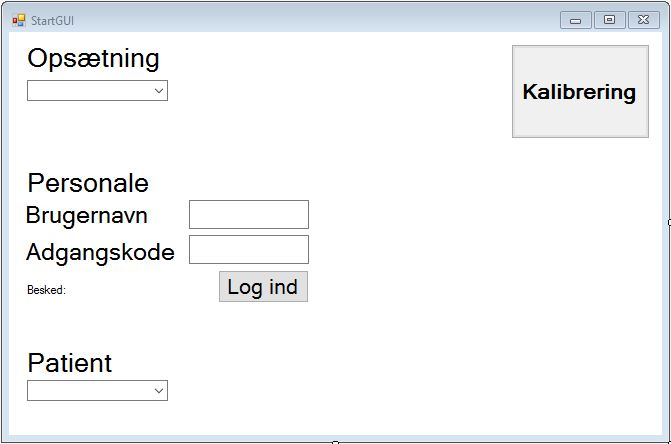
\includegraphics[width =0.5\textwidth , center]{billeder/skitseStart}
\caption{Skitse af startskærmen, hvilken repræsenterer EPJ systemet}
\end{figure}
\begin{figure}[h!]
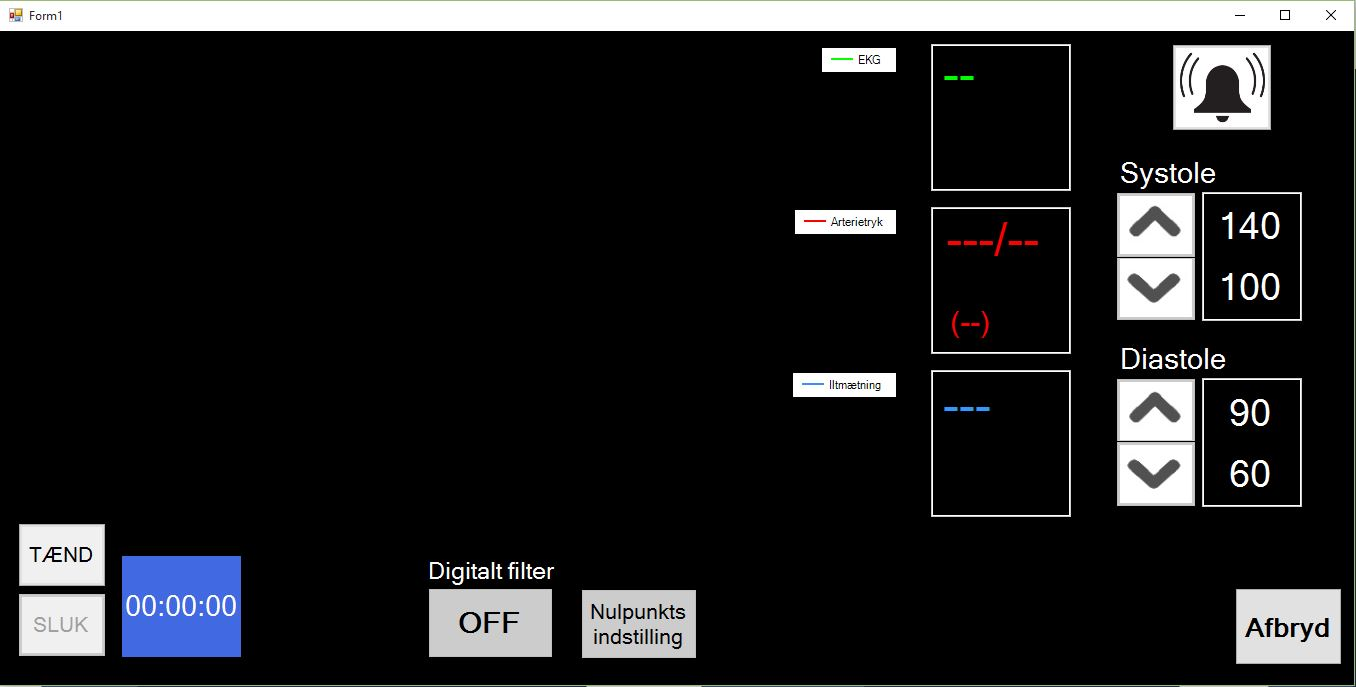
\includegraphics[width =1.0\textwidth , center]{billeder/skitseHoved}
\caption{Skitse af hovedskærmen, hvilken repræsenterer en blodtryksmåler}
\end{figure}
\end{enumerate}
\item \textbf{Reliability}
\begin{enumerate}
\item (\textbf{S}) INGEN RELIABILITY KRAV ENDNU
\end{enumerate}
\item \textbf{Performance}
\begin{enumerate}
\item (\textbf{S}) Tiden der går før måling af data påbegynder / vises i grafer må max være 2 sek.
\item (\textbf{M}) Tiden der går fra at data er analyseret til at data er gemt i database må være 2 sek. med en tolerance på +/-15\%  
\end{enumerate}
\item \textbf{Supportability}
\begin{enumerate}
\item (\textbf{M}) Softwaren skal være opbygget efter trelagsmodellen (Data-View-Model)
\end{enumerate}
\item \textbf{+ Test conditions}
\begin{enumerate}
\item (\textbf{M}) Der skal være adgang til en computer med Windows 7, 8 eller 10 - computeren skal minimum have 4 GB RAM.
\item (\textbf{M}) Der skal være adgang til en computer hvor National Instruments er installeret.
\end{enumerate}
\end{enumerate}

\chapter{Accepttest}
\section{Indledning}
\section{Accepttest for funktionelle krav}

\subsection{Opstilling}
Billede indsættes - haves ikke endnu

\begin{table}[H]
\caption{Accepttest for Use case 1}\label{tab:tabel8}
\begin{tabular}{|>{\raggedright\arraybackslash}p{2.5cm}| >{\raggedright\arraybackslash}p{2.9cm} | >{\raggedright\arraybackslash}p{2.9cm} | >{\raggedright\arraybackslash}p{2.9cm} | >{\raggedright\arraybackslash}p{2.8cm} |}
   \hline
   \textbf{Use case 1: Kalibrer apparat} &\textbf{Test}& \textbf{Prekondition} & \textbf{Forventet resultat} & \textbf{Godkendt/ kommentar}\\ \hline
   Normalforløb:& Tryk på "Kalibrering" & Blodtryksmåleren er tændt og tilsluttet kalibreringsudstyret. & Systemet er kalibreret og besked "Kalibreringen er fuldendt" vises på GUI & IKKE TESTBAR\\\hline
\end{tabular}
\end{table}

\begin{table}[H]
\caption{Accepttest for Use case 2}\label{tab:tabel8}
\begin{tabular}{|>{\raggedright\arraybackslash}p{2.5cm}| >{\raggedright\arraybackslash}p{2.9cm} | >{\raggedright\arraybackslash}p{2.9cm} | >{\raggedright\arraybackslash}p{2.9cm} | >{\raggedright\arraybackslash}p{2.8cm} |}
   \hline
   \textbf{Use case 2: Opsætning} &\textbf{Test}& \textbf{Prekondition} & \textbf{Forventet resultat} & \textbf{Godkendt/ kommentar}\\ \hline
   Normalforløb:& Tryk på opsætningens dropdown  & Systemet er tilsluttet en computer og er tændt & Liste med porte kommer frem. & \\\hline
   &Port vælges & Systemet er tilsluttet en computer og er tændt & Port valgt &\\\hline
\end{tabular}
\end{table}

\begin{table}[H]
\caption{Accepttest for Use case 3}\label{tab:tabel8}
\begin{tabular}{|>{\raggedright\arraybackslash}p{2.5cm}| >{\raggedright\arraybackslash}p{2.9cm} | >{\raggedright\arraybackslash}p{2.9cm} | >{\raggedright\arraybackslash}p{2.9cm} | >{\raggedright\arraybackslash}p{2.8cm} |}
   \hline
   \textbf{Use case 3: Log på} &\textbf{Test}& \textbf{Prekondition} & \textbf{Forventet resultat} & \textbf{Godkendt/ kommentar}\\ \hline
   Normalforløb:& Indtast brugernavn og kode & Port valgt & Systemet er kalibreret og besked "Kalibreringen er fuldendt" vises på GUI & \\\hline
   &Tryk "Login" & Port valgt & Den sundhedsfaglige er logget på &\\\hline
\end{tabular}
\end{table}


\begin{table}[H]
\caption{Accepttest for Use case 4}\label{tab:tabel8}
\begin{tabular}{|>{\raggedright\arraybackslash}p{2.5cm}| >{\raggedright\arraybackslash}p{2.9cm} | >{\raggedright\arraybackslash}p{2.9cm} | >{\raggedright\arraybackslash}p{2.9cm} | >{\raggedright\arraybackslash}p{2.8cm} |}
   \hline
   \textbf{Use case 4: Vælg patient} &\textbf{Test}& \textbf{Prekondition} & \textbf{Forventet resultat} & \textbf{Godkendt/ kommentar}\\ \hline
   Normalforløb:& Tryk på patient dropdown & Den sundhedsfaglige er logget på & Liste med patienter kommer frem  & \\\hline
   & Vælg patienten og dobbeltklik på denne & Den sundhedsfaglige er logget på & Hovedskærmen kommer frem &\\\hline
\end{tabular}
\end{table}


\begin{table}[H]
\caption{Accepttest for Use case 5}\label{tab:tabel8}
\begin{tabular}{|>{\raggedright\arraybackslash}p{2.5cm}| >{\raggedright\arraybackslash}p{2.9cm} | >{\raggedright\arraybackslash}p{2.9cm} | >{\raggedright\arraybackslash}p{2.9cm} | >{\raggedright\arraybackslash}p{2.8cm} |}
   \hline
   \textbf{Use case 5: Start signal} &\textbf{Test}& \textbf{Prekondition} & \textbf{Forventet resultat} & \textbf{Godkendt/ kommentar}\\ \hline
   Normalforløb:& Tryk på "Start"& Patient valgt & Systemet indhenter data og starter timer. EKG, arterietryk og iltmætningskurve præsenteres kontinuert på hver sin graf. Puls, systole, diastole, middeltryk og iltmætning vises som talværdier på GUI. -data gemmes automatisk i database & \\\hline
\end{tabular}
\end{table}

\begin{table}[H]
\caption{Accepttest for Use case 6}\label{tab:tabel8}
\begin{tabular}{|>{\raggedright\arraybackslash}p{2.5cm}| >{\raggedright\arraybackslash}p{2.9cm} | >{\raggedright\arraybackslash}p{2.9cm} | >{\raggedright\arraybackslash}p{2.9cm} | >{\raggedright\arraybackslash}p{2.8cm} |}
   \hline
   \textbf{Use case 6: Nulpunkts indstille signal } &\textbf{Test}& \textbf{Prekondition} & \textbf{Forventet resultat} & \textbf{Godkendt/ kommentar}\\ \hline
   Normalforløb:& Tryk på "Nulpunkts indstilling" & Signalet er startet & Besked " Nulpunkts indstilling er fuldendt" vises på GUI &\\\hline
\end{tabular}
\end{table}


\begin{table}[H]
\caption{Accepttest for Use case 7}\label{tab:tabel8}
\begin{tabular}{|>{\raggedright\arraybackslash}p{2.5cm}| >{\raggedright\arraybackslash}p{2.9cm} | >{\raggedright\arraybackslash}p{2.9cm} | >{\raggedright\arraybackslash}p{2.9cm} | >{\raggedright\arraybackslash}p{2.8cm} |}
   \hline
   \textbf{Use case 7: Udsæt alarm } &\textbf{Test}& \textbf{Prekondition} & \textbf{Forventet resultat} & \textbf{Godkendt/ kommentar}\\ \hline
   Normalforløb:& Tryk på "Udsæt alarm" & Alarmering er startet & Systemet stopper alarmens lyd i et minut &\\\hline
\end{tabular}
\end{table}

\begin{table}[H]
\caption{Accepttest for Use case 8}\label{tab:tabel8}
\begin{tabular}{|>{\raggedright\arraybackslash}p{2.5cm}| >{\raggedright\arraybackslash}p{2.9cm} | >{\raggedright\arraybackslash}p{2.9cm} | >{\raggedright\arraybackslash}p{2.9cm} | >{\raggedright\arraybackslash}p{2.8cm} |}
   \hline
   \textbf{Use case 8: Digitalt filter } &\textbf{Test}& \textbf{Prekondition} & \textbf{Forventet resultat} & \textbf{Godkendt/ kommentar}\\ \hline
   Normalforløb:& Tryk på "Digitalt filter OFF" & Signalet er startet & Systemet slår det digitale filter fra. Data er ufiltreret og knappen ændrer navn &\\\hline
   &Tryk på "Digitalt filter ON" & Signalet er startet & Systemet slår det digitale filter til. Data er filtreret og knappen ændrer navn. &\\\hline
\end{tabular}
\end{table}


\begin{table}[H]
\caption{Accepttest for Use case 9}\label{tab:tabel8}
\begin{tabular}{|>{\raggedright\arraybackslash}p{2.5cm}| >{\raggedright\arraybackslash}p{2.9cm} | >{\raggedright\arraybackslash}p{2.9cm} | >{\raggedright\arraybackslash}p{2.9cm} | >{\raggedright\arraybackslash}p{2.8cm} |}
   \hline
   \textbf{Use case 9: Juster systolens grænseværdi } &\textbf{Test}& \textbf{Prekondition} & \textbf{Forventet resultat} & \textbf{Godkendt/ kommentar}\\ \hline
   Normalforløb:& Tryk på "Systole op"& Signalet er startet & Grænseværdien ændres 2.5 mmHg op og intervellet vises i GUI &\\\hline
   &Tryk på "Systole ned" & Signalet er startet & Grænseværdien ændres 2.5 mmHg ned og intervallet vises i GUI & \\\hline
\end{tabular}
\end{table}

\begin{table}[H]
\caption{Accepttest for Use case 10}\label{tab:tabel8}
\begin{tabular}{|>{\raggedright\arraybackslash}p{2.5cm}| >{\raggedright\arraybackslash}p{2.9cm} | >{\raggedright\arraybackslash}p{2.9cm} | >{\raggedright\arraybackslash}p{2.9cm} | >{\raggedright\arraybackslash}p{2.8cm} |}
   \hline
   \textbf{Use case 10: Juster diastolens grænseværdi } &\textbf{Test}& \textbf{Prekondition} & \textbf{Forventet resultat} & \textbf{Godkendt/ kommentar}\\ \hline
   Normalforløb:& Tryk på "Diastole op"& Signalet er startet & Grænseværdien ændres 2.5 mmHg op og intervellet vises i GUI &\\\hline
   &Tryk på "Diastole ned" & Signalet er startet & Grænseværdien ændres 2.5 mmHg ned og intervallet vises i GUI & \\\hline
\end{tabular}
\end{table}

\begin{table}[H]
\caption{Accepttest for Use case 11}\label{tab:tabel8}
\begin{tabular}{|>{\raggedright\arraybackslash}p{2.5cm}| >{\raggedright\arraybackslash}p{2.9cm} | >{\raggedright\arraybackslash}p{2.9cm} | >{\raggedright\arraybackslash}p{2.9cm} | >{\raggedright\arraybackslash}p{2.8cm} |}
   \hline
   \textbf{Use case 11: Alarmer } &\textbf{Test}& \textbf{Prekondition} & \textbf{Forventet resultat} & \textbf{Godkendt/ kommentar}\\ \hline
   Normalforløb:& Grænseværdi overskrides& Signalet er startet & Alarm starter med lyd og tallet, hvis grænseværdi er overskredet, blinker &\\\hline
\end{tabular}
\end{table}

\begin{table}[H]
\caption{Accepttest for Use case 12}\label{tab:tabel8}
\begin{tabular}{|>{\raggedright\arraybackslash}p{2.5cm}| >{\raggedright\arraybackslash}p{2.9cm} | >{\raggedright\arraybackslash}p{2.9cm} | >{\raggedright\arraybackslash}p{2.9cm} | >{\raggedright\arraybackslash}p{2.8cm} |}
   \hline
   \textbf{Use case 12: Stop signal } &\textbf{Test}& \textbf{Prekondition} & \textbf{Forventet resultat} & \textbf{Godkendt/ kommentar}\\ \hline
   Normalforløb:& Tryk på "Stop" & Signalet er startet & Signalet og timer stopper &\\\hline
\end{tabular}
\end{table}

\begin{table}[H]
\caption{Accepttest for Use case 13}\label{tab:tabel8}
\begin{tabular}{|>{\raggedright\arraybackslash}p{2.5cm}| >{\raggedright\arraybackslash}p{2.9cm} | >{\raggedright\arraybackslash}p{2.9cm} | >{\raggedright\arraybackslash}p{2.9cm} | >{\raggedright\arraybackslash}p{2.8cm} |}
   \hline
   \textbf{Use case 13: Afbryd signal } &\textbf{Test}& \textbf{Prekondition} & \textbf{Forventet resultat} & \textbf{Godkendt/ kommentar}\\ \hline
   Normalforløb:& Tryk "Afbryd" & Signalet er stoppet & Pop-up vindue kommer op: "Er du sikker?" &\\\hline
   &Tryk "Ja"&Signalet er stoppet& Startskærmen kommer frem og ny måling kan foretages &\\\hline
\end{tabular}
\end{table}



\newpage

\newpage

\newpage

\section{Accepttest for ikke-funktionelle krav}

\begin{longtable}{|>{\raggedright\arraybackslash}p{1.1cm}| >{\raggedright\arraybackslash}p{2.7cm} | >{\raggedright\arraybackslash}p{2.7cm} | >{\raggedright\arraybackslash}p{2.7cm} | >{\raggedright\arraybackslash}p{2.2cm} |>{\raggedright\arraybackslash}p{2.2cm}|}
   \caption{Accepttest for ikke-funktionelle krav}\label{tab:label13}
\\ \hline   
\textbf{Krav nr.}&\textbf{Krav} &\textbf{Test}& \textbf{Forventet resultat} & \textbf{Resultat} & \textbf{Godkendt/ kommentar}\\ \hline
  1.1 & Programmet skal have et digitalt filter til udglatning af blodtrykssignal & & & & \\\hline
  1.2 & Programmet skal give alarm når grænseværdier overskrides med lyd og hvor den overskredede grænse værdi blinker på skærmen. & & & & \\\hline
  1.3 & Programmet skal kunne gemme blodtrykssignalet i en database & & & & \\\hline\hline
  2.1 & Programmet skal have to window form: startskærm,der fungerer som EPJ systemet, og hovedskærm, hvilken fungerer som selve blodtryksmåleren & & & & \\\hline
  2.2 & Programmet skal have en "Login" knap på startskærmen & & & & \\\hline
  2.3 & Programmet skal have ne "Kalibrering" knap på startskærmen & & & & \\\hline
  2.4 &Sundhedsfaglig personale skal kunne ændre "device/enhedsnavn" i dropdown på startskærm & & & & \\\hline
  2.5 & Programmet skal indeholde en dropdown, hvor patienten kan vælges på startskærmen & & & & \\\hline
  2.6 & Programmet skal have en "Nulpunkts indstilling" knap på hovedskærmen & & & & \\\hline
  2.7 & Programmet skal have en knap, til at slå det digitale filter fra og til, på hovedskærmen & & & & \\\hline
  2.8 & Programmet skal have knapper, til at justere systolisk og diastolisk grænseværdiintervaller op og ned, på hovedskærmen & & & & \\\hline
  2.9 & Programmet skal have en "Udsæt alarm" knap på hovedskærmen & & & & \\\hline
  2.10 & Programmet skal have en "Tænd" knap på hovedskærmen & & & & \\\hline
  2.11 & Programmet skal have en "Sluk" knap på hovedskærmen & & & & \\\hline
  2.12 & Programmet skal have en "Afbryd" knap på hovedskærmen & & & & \\\hline
  2.13 & Teksten på startskærmen skal kunne aflæs fra 1 meters afstand med en synsstyrke i intervallet +/-1 & & & & \\\hline
  2.14 & Teksten og graferne på hovedskærmen skal kunne læses fra 2 meters afstand ved synsstyrke i intervellet på +/-1 & & & & \\\hline
  2.15 & Programmet skal præsentere grafer efter standard & & & & \\\hline
  2.16 & Programmet skal præsentere data i tal efter standard & & & & \\\hline\hline
  3.1 & Ingen krav endnu & & & & \\\hline\hline
  4.1 & Tiden der går før målingen af data påbegynder/vises i grafer må maksimalt være 2.0 sek. & & & & \\\hline
  4.2 & Tiden der går fra at data er analyseret til at data er gemt i database må være 2.0 sek. med en tolerance på +/- 15\% & & & & \\\hline\hline
  5.1 & Softwaren skal være opbygget efter trelagsmodellen & & & & \\\hline\hline
  6.1 & Der skal være adgang til en computer med Windows 7, 8 eller 10 - computeren skal minimum have 4 GB RAM & & & & \\\hline
  6.2 & Der skal være adgang til en computer hvor National Instruments er installeret & & & & \\\hline
\end{longtable}

\section{Godkendelses formular}
\begin{table}[h!]
\label{tab:tabel14}
\begin{tabular}{| l | >{\raggedright\arraybackslash}p{12cm} |}
   \hline
   \textbf{Dato for test} &\\ \hline
   \textbf{Godkendes af:} & \\ \hline
\end{tabular}
\end{table}
\textbf{Ved underskrivelse af dette dokument godkendes den kørte accepttest}
\newline
\textbf{Sted og dato:}\\
\\
\\
\begin{table}
[h!]
\begin{tabular}{ l lllllllll l}
--------------------------------------&&&&&&&&&&--------------------------------------\\ 
Kundens underskrift &&&&&&&&&&Leverandørens underskrift\\
\end{tabular}
\end{table}